%Chapter 2

\renewcommand{\thechapter}{2}

\chapter{Literature Review}

\section{Statement of Purpose}
While EVs have not been universally adopted yet, they have come a long way since their inception into the 
automotive market. This can be attributed to enhanced charging methods coupled with increased range. 
The goal of this research has been to contribute to the current trend by testing technology that makes 
EVs more convenient than internal combustion engine (ICE) vehicles in an effort to propel mass adoption 
of a more sustainable alternative. By creating a model that optimizes dynamic wireless power transfer 
(DWPT) on motorways, we will assist other researchers in this field in determining the most energy and 
cost efficient design. In turn, this will help lead to the physical implementation of this design in 
motorways across the world, practically eliminating the need to stop and charge. This would effectively 
eliminate arguably the largest downside of switching to an electric vehicle (EV) from an ICE vehicle.	

\section{Background on EVs}
Most EVs of the modern era are driven by an electric motor that draws power from an onboard battery. 
These engines produce instantaneous torque and are much more efficient than their ICE counterparts.  
The most commonly used battery types are lithium ion, lead-acid, and nickel metal-hydride batteries, 
with lithium ion yielding the best performance and efficiency characteristics \cite{eberhard_21_2007}.  
As a result, more manufacturers are implementing their EVs with lithium-ion batteries.  In non-hybrid EVs 
which only rely on batteries for power, charging is done by plugging in a source of electricity to the vehicle.  
That means that these vehicles can be “charged at home from a standard outlet or on a corporate car park” 
\cite{clement-nyns_impact_2010}.  Although the location of the charge may be more convenient, 
the time it takes to reach full energy capacity is not.  With each charge lasting anywhere from thirty minutes 
to eight hours, electric charging takes considerably more time than a quick stop at the gas station. A switch 
to EVs with a one-hundred-mile-range would not change day to day driving patterns for a significant population, 
needing only to charge the car at home overnight \cite{pearre_electric_2011}. The problem arises 
when traveling longer distances. A limited driving range, a lack of a well-established EV infrastructure, and 
inefficient charging times provide ample reason as to why EVs have not entirely caught on yet.

\section{Physics}
\label{sec: s2.3}
This section will provide a brief overview of the physics principles that DWPT relies on. 
DWPT would not be possible without the natural phenomena of magnetic induction and magnetic resonance. 
The equations in this section will serve as a starting point for our mathematical model, so they are 
important to understand.  

\subsection{Electric Circuits}
When discussing the internal components of EVs, or even typical vehicles, concepts such as voltage and 
power are crucial to understanding how they work, especially when focused on aspects of charging. 
Voltage represents the potential difference in charge between two points; the greater the voltage, 
the greater the amount of charge that passes through a point per unit of time. Symbolically, 1 V = 1 J/C 
\cite{young_university_2016}. This means that a 1-volt battery will move 1 joule of energy per coulomb of charge. 
Closely related to voltage is the concept of current: current is the flow of electric charge. 
This is represented with the unit of ampere (A), where 1 A = 1 C/s. This means that one ampere stands for 
the flow of one coulomb of charge per second through a point.  Together, voltage and current (as well as 
electrical resistance) have a fundamental relationship which can be demonstrated by Ohm’s Law: V = IR
\cite{young_university_2016}. Voltage and current are proportionally related, where R is simply the resistance 
of the system, or the opposition of current flow. The unit for resistance is ohm ($\Omega$). Power, represented with 
P (the unit is watts: 1 W = 1 J/s), stands for the rate of energy transferred per unit of time. Mathematically, 
power can be found with the formula P = IV \cite{young_university_2016}. In other words, power represents the 
flow of joules per second -- the same value of power can be achieved by a large amount of charge flowing 
slowly or a small amount of charge which flows quickly.

In the simplest terms, voltage is how “hard” electricity is pushed, current is how much charge is flowing 
through a wire, and power is energy over time.

\subsection{AC and DC Current}
As stated previously, current is the flow of electric charge. However, the flow of charge can have different 
states: simply put, current can be a continuous flow in one direction (DC - direct current) or a continuously 
oscillating flow of “pulling and pushing” charge (AC - alternating current) \cite{young_university_2016}. 
Typically, confusion arises when distinguishing between the applied benefits, or differences, of the two types. 
Ultimately, AC is used when transmitting large amounts of power over large distances. Energy losses, such 
as heat, are proportional to the current, but not the voltage. Therefore, to transfer a large amount of power, 
voltage is set very high, and current low to minimize loss. However, large voltages are dangerous for typical 
consumers, so the power has to be converted again before arriving at homes and buildings. If DC is used for 
power transfer, there would be no easy way to change the voltage, but with AC, a transformer can be used to 
convert the power easily \cite{young_university_2016}. Aside from transmitting power, AC is used whenever changing 
magnetic fields are desired, such as with a transformer. The mechanism behind a transformer is related to induction, 
which will be described in the next section \cite{young_university_2016}.

\subsection{Magnetic Fields}
Magnetic fields surround moving charges.  For wireless power transfer (WPT), we consider moving charge in the form 
of a current in a solenoid, or circular coil of wire with N windings.  The magnetic field of a solenoid can be 
described by the equation:
\begin{equation}
    B = \mu NI
\end{equation}
where B is the magnetic field measured in Teslas, µ is the permeability of the material, N is the number of windings 
of the coil, and I is the current in Amperes \cite{young_university_2016}. Looking at the coil from above as it lays 
flat, the field points upward if the current flows counterclockwise and downward if the current flows clockwise, 
according to the right-hand rule.  

\subsection{Magnetic Flux}
Magnetic flux is a measure of the flow of a magnetic field through a closed surface. Magnetic flux can be described 
by the equation:
\begin{equation}
    \Phi_B = \int{\vec{B} \cdot d\vec{A}}
\end{equation}
where $\Phi_B$ is the magnetic flux and $d\vec{A}$ is the vector element of surface area \cite{young_university_2016}. 
This equation can be simplified to 
\begin{equation}
    \Phi_B = BA cos(q)
\end{equation}
given that the magnetic field is uniform, the surface is flat, A is area and  is the angle between the field and 
the normal to the surface \cite{young_university_2016}. Figure \ref{fig: f1} further explains this relationship 
\cite{young_university_2016}. If the surface and field are not perpendicular, then less of the magnetic field lines 
pass through it. Likewise, if theta is zero, the magnetic flux is at a maximum.  

\begin{figure}
    \begin{center}
    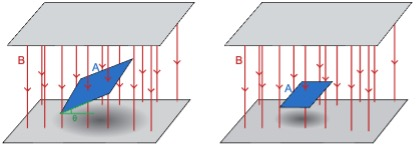
\includegraphics[width=5in]{fig1.jpg}
    \end{center}
    \renewcommand{\baselinestretch}{1}
    \small\normalsize
    \begin{quote}
    \caption[Magnetic Flux]{Magnetic Flux \cite{noauthor_what_nodate}.} \label{fig: f1}
    \end{quote}
\end{figure}

\subsection{Electromagnetic Induction}
Induction is the main principle on which WPT relies. Faraday’s law of electromagnetic induction says that changing 
magnetic flux can induce an electromotive force (EMF) in a circuit:
\begin{equation}
    \mathcal{E} = -\frac{d\Phi_B}{dt}
\end{equation}
For example, when a current flows through a coil of wire, it creates a magnetic field.  If another object such as 
the receiving coil of wire comes into close range with the magnetic field, a current is induced in it momentarily 
\cite{young_university_2016}. However, if the current in the receiving coil continues to change in time, so does 
the magnetic field, and this changing magnetic field is able to sustain an AC current in the receiving coil 
\cite{young_university_2016}. It can be said that the transmitting coil is inducing an AC current in the receiving coil.  

Nikola Tesla discovered that electromagnetic induction could be used to seemingly transfer power through the air 
in the late 1800s \cite{lu_wireless_2016}.  Simple radio antennas have functioned via this method 
of power transfer since Tesla’s time, but until recently, it has not been used in cars and other electronics 
like Tesla had originally hoped \cite{lumpkins_nikola_2014}.  This is because the efficiency of this charging method over 
long distances or for larger applications did not appear to be economical, but with recent research the efficiency 
has been proved to be higher than originally thought \cite{lu_wireless_2016}.  

\subsection{AC to DC Current Conversion}
In order to charge a battery, a DC current is necessary, but the induced current is an AC current. 
A circuit element called a diode is necessary to convert AC current into pulses of DC current. 
A diode is a device with two terminals that only allows current to flow in one direction \cite{young_university_2016}. 

A rectifier is a more sophisticated version of a diode that is necessary in complex circuitry like that of EVs. 
The simplest of rectifiers, a single-phase half-wave rectifier, allows only the positive part of a sinusoidal AC 
current to pass through and into the battery \cite{skvarenina_power_2001}.  Single-phase full-wave rectifiers are able to 
convert the positive part of the sinusoidal AC current and the inverted negative part of the sinusoidal AC current 
into DC current \cite{skvarenina_power_2001}.  As shown in Figure \ref{fig: f2}, it is far more complicated and requires the use of four 
diodes. 

\begin{figure}
    \begin{center}
    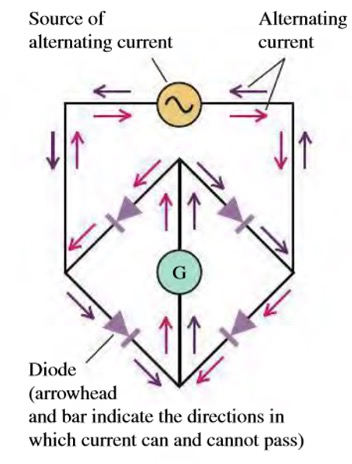
\includegraphics[width=3in]{fig2.jpg}
    \end{center}
    \renewcommand{\baselinestretch}{1}
    \small\normalsize
    \begin{quote}
    \caption[A DC current is established across the galvanometer]{A DC current is established across the galvanometer (represented by the G) \cite{young_university_2016}} \label{fig: f2}
    \end{quote}
\end{figure}

\subsection{Magnetic Resonance}
A transmitting coil (or circuit) can be designed so that its resonant frequency is the same as the frequency of 
the AC current in the transmitting circuit, inducing a current in the receiving circuit that has the greatest 
amplitude (meaning the greatest EMF) \cite{young_university_2016}. As shown in Figure \ref{fig: f3}, the amplitude greatly 
increases near the natural oscillating frequency. The natural oscillation frequency of the circuit can be manipulated 
by changing the strength of various circuit elements such as inductors, capacitors and resistors, or by changing the 
number of windings in the coil.  Alternatively, the current in the transmitting coil can be chosen based on a known 
natural oscillation frequency of the receiving circuit.

\begin{figure}
    \begin{center}
    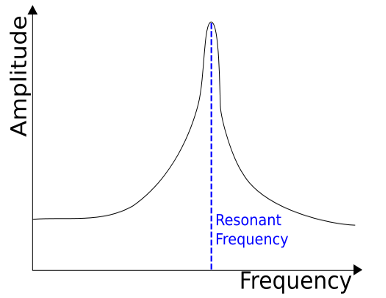
\includegraphics[width=3in]{fig3.png}
    \end{center}
    \renewcommand{\baselinestretch}{1}
    \small\normalsize
    \begin{quote}
    \caption[Voltage Amplitude vs. Frequency]{Voltage Amplitude vs. Frequency \cite{noauthor_resonant_nodate}.} \label{fig: f3}
    \end{quote}
\end{figure}

\section{Existing Methods}
\subsection{Wireless / DWPT Charging}
DWPT will allow EVs to drive further without having to stop to charge the battery for an extended period of time. 
Many companies are already researching ways of wirelessly charging batteries for devices. A thorough review of 
existing research was conducted prior to determining our research’s focus.

\subsection{Stationary Wireless Charging }
Stationary wireless charging is one method of charging currently being tested. Stationary charging is when the 
vehicle has a charging pad mounted on its underside and the driver parks overtop of the charging pad on the floor. 
This allows a signal to be picked up between the two pads and charges the vehicle 
\cite{fisher_electric_2014}. Energy is converted from AC to DC using a power converter which then 
transfers the energy back to the battery bank. The charging time of using stationary wireless charging depends on a 
variety of different variables including the source power level, charging pad sizes, and air-gap distance between 
the two windings \cite{panchal_review_2018}. These stationary wireless charging stations can also be installed 
in parking garages, homes, park ‘n’ ride facilities or even shopping centers. This type of wireless charging 
alleviates the hassle for the consumer because they do not have to worry about forgetting to plug in their car at 
night or dealing with trying to plug their car in if it is raining outside. This stationary charging technique is 
being applied to public transportation systems. For example, electric busses are trying this because they take an 
extended period of time to load and unload passengers at stops. They can gain some power to charge their batteries 
from these stationary pads at bus stops. This is known as “opportunity charging” \cite{lukic_cutting_2013}. 
This will allow electric city buses to cut down on their battery sizes and in turn their weight. Using this same 
technology could potentially reduce the size of heavy batteries in EVs. 

There have been numerous stationary wireless charging prototypes designed, each one with the location of the 
charging pad in different areas of the car such as the front, rear, and center of the car. Evatran is a company 
working on “Plugless Power” for passenger cars with the receiver pad location in the front of the car. With their 
prototype they can achieve an air gap distance of 102 mm with an efficiency of 90\% power transfer 
\cite{panchal_review_2018}. This company is just one of the many that are researching the stationary wireless 
power transfer, but overall, the prototypes have been developed with an air-gap distance of 100-300 mm with an 
efficiency from 71 to 95\% \cite{panchal_review_2018}. 

\subsection{Dynamic Wireless Power Transfer (DWPT)}
\label{sec: s2.4.3}
DWPT is when a vehicle is moving and picking up a charge simultaneously. This usually involves a charging pad with 
coils connected to the bottom of the vehicle and another set of charging pads with coils underneath the road that 
are each activated for a split second as the vehicle passes over it \cite{fisher_electric_2014}.  
This could potentially transfer power from a non-moving transmitter, like the pad underneath the road, to the 
receiver coil of a moving object, like the vehicle. Many issues arise with DWPT systems, like low power transfer 
efficiency, and the considerable power loss that occurs \cite{rakhymbay_precise_2018}. Currently, a University of Auckland 
research team has designed a prototype of a 400 m long stretch of track that wirelessly transmits 100 kW of power 
to a train \cite{rakhymbay_precise_2018}. Another team from the Oak Ridge National Laboratory has proven that the 
efficiency of the power transfer of a DWPT system depends on the position of the transmitter coil with respect to the 
pickup coil \cite{rakhymbay_precise_2018}. What this essentially means is that the position that a vehicle travels overtop 
of the coils in the road greatly impacts how much power can be drawn. To minimize this problem of power loss due to 
lateral misalignment there have been many methods proposed to maximize the lateral misalignment tolerance. These 
methods include changing the geometry of the coil, placing multiple coils in an orthogonal configuration, overlapping 
the configuration of the coils, or using different geometry of several different coils in one unit 
\cite{karam_hwang_autonomous_2017}. 

At this time, circular coils and Double D (DD) coils are the common type for the pad arrays. DD coils have a 
higher coupling coefficient and a higher offset tolerance \cite{xiang_design_2017}. This means 
that you get a higher fraction of magnetic flux produced by the DD coils compared to the circular coils. 
There is a new design of DD coils proposed that uses DD coils in a crossed design as shown in Figure \ref{fig: f4}. 
Unlike the original, the crossed DD design will offset the coils so that the edges are not flushed against each other. 
The results concluded that when the conventional DD coil is chosen as the primary pad type the average output of 
power was 7.1528 kW and the efficiency was 84.02\% and when the crossed DD was chosen the average output of power 
was 11.517 kW and the efficiency was 91.79\% \cite{xiang_design_2017}. The report concluded that 
26\% more energy can be transferred while using DWPT with this crossed DD design of the coils \cite{karam_hwang_autonomous_2017}. 

\begin{figure}
    \begin{center}
    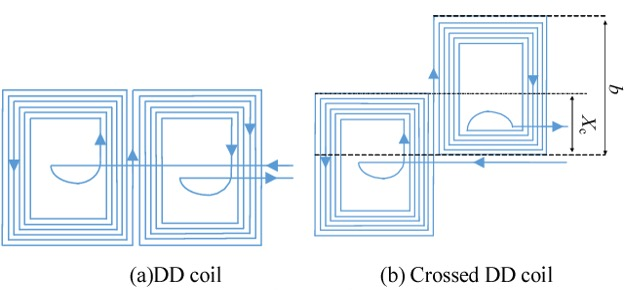
\includegraphics[width=5in]{fig4.jpg}
    \end{center}
    \renewcommand{\baselinestretch}{1}
    \small\normalsize
    \begin{quote}
    \caption[Difference between the alignment of DD coils and the crossed DD coils]{Difference between the alignment of DD coils and the crossed DD coils \cite{xiang_design_2017}.} \label{fig: f4}
    \end{quote}
\end{figure}

For maximum efficiency of power transfer in DWPT the vehicle has to be aligned on the road in the right orientation. 
Misalignment of the vehicle is inevitable since a person is physically driving and controlling the vehicle. 
A proposed method to change this is to use an autonomous coil alignment system for EVs that will detect misalignment 
and then the lateral position of the EV would be self-adjusted by an autonomous steering function 
\cite{karam_hwang_autonomous_2017}. 

\subsection{Magnetic Resonance Coupling}
Magnetic resonance coupling is another technique companies are using to wirelessly charge batteries. 
With this method there are two different resonators. One of the resonators receives energy from an 
external power supply while the other resonator is physically separated from the first and is used to 
supply working power to an external load \cite{ho_comparative_2011}. Both of these resonators are trying 
to oscillate at the same resonant frequency to produce the greatest amplitude. This transfers non-radiative 
energy between both resonators through coupling of the resonant-field evanescent tails \cite{ho_comparative_2011}. 
An evanescent field is an oscillating electric field in which the energy is spatially concentrated around the source, 
so this essentially takes the non-radiative energy and couples it with the oscillating electric field. Using a pair 
of rectangular spiral copper windings with the same shape and structure can help achieve efficient wireless energy 
transfer. With this system the receiver output voltage decreases linearly with an increase in the distance between 
the transmitter coil and the receiver coil \cite{ho_comparative_2011}. The main company that is researching this 
type of DWPT is Witricity. Using this method of magnetic resonant coupling, DWPT can have an efficiency of 90\% 
and a power transfer rate of up to 3.3 kW. What this essentially means is that the electromagnetic waves produced 
by the resonators can be used to transfer energy. To ensure that this works and that resonant objects can exchange 
energy efficiently, the correct resonant frequency has to be calculated. There are many benefits to using this 
technique to charge objects wirelessly. With magnetic resonance coupling you can get long transmission distance 
and no radiation, but it is difficult to adjust the resonant frequency if you are trying to charge multiple devices 
or objects \cite{parmesh_wireless_2017}. Magnetic resonance is currently being used to wirelessly charge phone 
batteries, but the research done on the different coil shapes, sizes, and their efficiency can still be used to guide 
our research on wirelessly charging EVs.

\section{Limitations}
\subsection{Safety}
The most significant safety limitation related to DWPT is electromagnetic field exposure. The medical community is 
somewhat split on categorizing the effects of electromagnetic field exposure as either beneficial or detrimental to 
human health. There are claims that applications of electromagnetic fields, even those generated from cellphones, 
have cognitive benefits \cite{arendash_electromagnetic_2010}. Other experts warn that electromagnetic field exposure could promote 
cancer and increase risk of miscarriage \cite{kostoff_combined_2013}. While the levels for which electromagnetic fields are 
considered beneficial or harmful are unestablished, the International Commission on Non-Ionizing Radiation Protection 
(ICNIRP) sets 6.25 µT as the acceptable limit for the public.  The Oak Ridge National Laboratory measured the 
electromagnetic field at 9 different positions above a wireless power transmitter coil and found that it peaked at 
about half the allowable limit for 8 of the 9 positions \cite{onar_novel_2013}. For the one position where the measured 
electromagnetic field was over 3 times the allowable, a strategically placed thin aluminum sheet brought it down to 
just under 6 µT \cite{onar_novel_2013}. While electromagnetic field exposure is a concern that can easily be remediated, 
the possible effects of an induced magnetic field on medical devices such as pacemakers may be harder to manage.

In simple terms, pacemakers are medical devices that help regulate the heartbeat, typically implanted after some 
heart-related emergency. Because they are electronic, they are susceptible to being adversely affected by magnetic 
fields. If a pacemaker were to act irregularly due to electromagnetic field exposure, it could cause significant 
health issues or even death for the user. A study published in the medical journal EP Europace examined the effects 
of electromagnetic fields on pacemakers and implantable cardioverter-defibrillators (ICDs). They found that even at 
levels of 300 µT, no noticeable or detrimental effects were detected on the implanted devices 
\cite{tiikkaja_electromagnetic_2013}. As mentioned before, in experimental trials of DWPT, the measured electromagnetic 
field remained at about 1\% of that used in the medical trial.

Electromagnetic field exposure is a safety concern that should be monitored but should not prevent the implementation 
of DWPT in public roads. The electromagnetic fields generated are not expected to exceed the safe limit for the public 
and will not pose a threat to those with implanted medical devices. Electromagnetic shielding – the use of a material 
to block an electromagnetic field – is possible, as demonstrated by the Oak Ridge lab in their DWPT trial. Graphene 
foam composites are most efficient for shielding, having a high shielding effectiveness and desirable material 
properties, such as being lightweight and flexible \cite{chen_lightweight_2013}. The implementation of electromagnetic 
shielding could increase the cost of constructing a DWPT road. When analyzing the economics of implementation, 
this is something that would need to be considered.

\subsection{Cost of Implementation}
The cost of full-scale implementation is generally calculated from a design perspective, as DWPT is still in testing 
and development. The factors that must be taken into consideration are the coils of an optimized size required to 
charge an EV, the cost of removing the road to install the coils, and the cost of repaving the road after installation 
\cite{chen_lightweight_2013}. Costs could be reduced by implementing DWPT into roads that are already in need of repaving. 
Furthermore, the energy required to keep such coils powered throughout the day must also be considered, making sure 
that peak hours are given extra energy to compensate for increased vehicular traffic \cite{chen_lightweight_2013}. 
The following analysis of cost will be qualitative, as not much research has been done on the quantitative cost. 

The length of individual coils must be calculated empirically. However, as mentioned previously, full scale 
implementation is still novel and companies who have obtained successful results are reluctant to share their 
findings. The total raw material cost would consist of the length required for each coil multiplied by the number 
of coils installed over the given length of road. Infrastructure costs will vary, depending on the chosen power supply. 
For solar power, the installation costs of solar panels must be taken into consideration. What must be determined is 
the number of coils that can be powered per solar panel \cite{chen_lightweight_2013}). If an alternative source of power is used, 
the cost of that power must be determined. 

Furthermore, a significant portion of the cost of implementation will be the physical installation of the coils. 
For initial implementation, one charging lane per highway would be sufficient, given the current usage rates of 
EVs \cite{li_longitudinal_2018}. Depending on the length of road used, the cost of removing the pavement and repaving the 
road after installation could outweigh the benefits of implementing wireless power transfer. As interstate 
highways are maintained by the state government, it is possible that some toll would be needed to fund a project 
of this magnitude. Still, some companies may not be convinced that the benefits of dynamic wireless power transfer 
outweigh the initial capital requirements \cite{chen_lightweight_2013}. 

Something that must be taken into consideration when implementing a DWPT lane on the roads is the change in traffic. 
Simulations have shown that having a DWPT lane can impact traffic in a negative manner \cite{li_longitudinal_2018}. EVs with 
lower battery charge will drive in the charging lane at a slower pace than other cars around them \cite{li_longitudinal_2018}. 
If a vehicle is going slow in a wireless charging lane, its battery will be more charged \cite{li_longitudinal_2018}. 
This is because the vehicle is spending more time in the charging lane and is not utilizing as much power. 
However, there are possible ways to alleviate this problem. One solution to this problem would be to require 
that cars be at a specific battery charge to be able to use the charging lane \cite{li_longitudinal_2018}. 
This will ensure that vehicles will not go slower in the charging lane. Additionally, there will be a significantly 
larger amount of traffic when actually constructing the lanes, which will take time to complete.

Another consideration when implementing a DWPT lane on the roads is the cost. The initial construction cost of 
implementing a DWPT lane would be about \$200/m or \$321,900/mi \cite{chen_lightweight_2013}. However, this is just an 
estimate and actual costs will vary. The expenses of road maintenance and providing the coils with power will be 
higher than a traditional road, which may require a toll on the DWPT lane similar to what we see on some HOV lanes 
on Interstates currently. There are many factors that need to be considered when implementing a DWPT lane. 
A charging station costs significantly less, but a DWPT lane is much more efficient, in terms of time, 
for an EV than charging stations. 

The design of the DWPT lane system will consist of several components. Two of the most important components are 
the transmitter and receiver coil \cite{throngnumchai_design_2013}. The transmitter coil will be on the road while 
the receiver coil will be on the EV (so that the vehicle will be able to receive the magnetic field emitted 
from the receiver coil). It is important that we shield the body of the EV from the magnetic field, so there 
will be material to differentiate the vehicle and receiver coil \cite{throngnumchai_design_2013}. Typically, asphalt 
concrete is used to construct roads. However, that material may damage the coil or reduce power transfer efficiency 
due to low permeability of the material. It is important to look at alternative concretes to make sure the transmitter 
coil stays intact. There are many variables to consider when designing a DWPT lane. Examples include different coil 
variables, how far apart the different coil circuits should be, what to put in the coil circuits to maximize power 
transfer, what road material to use, etc. \cite{panchal_review_2018}. The goal is to maximize power transfer 
efficiency and reduce cost.

\section{Conclusion}
EVs are the future of the transportation industry because they are a feasible solution to slow global warming by 
reducing CO2-equivalent emissions by 80\% \cite{helmers_electric_2012}. At present, the most significant limitation to 
EV use is the power system because of charging time and short range. If DWPT technology can be applied in the future, 
charging EVs will be much more convenient and require much less time. As a result, EVs will be a preferable option 
for drivers with all needs including long-distance travels.

The goal of our research has been to add to this volume of work by thoroughly studying the possible issues regarding 
safety, implementation, and other areas of DWPT for EVs. Our goal has been to find the optimized design of a system 
with maximization of electrical efficiency and cost-efficiency using DC power because research in use of DC power 
for this application is not as extensive. Developing a DWPT system using DC power with a high enough efficiency and 
low enough cost will enable EVs to become a feasible and attractive option for all drivers. 